\RequirePackage[abort, l2tabu, orthodox]{nag}
\documentclass[pageno]{jpaper}

% standard LaTeX packages that do not interfere with hyperref
\usepackage{alltt}
\usepackage{amssymb}
\usepackage{booktabs}
\usepackage{caption}
\usepackage[draft]{fixme}
\usepackage{epstopdf}
\usepackage{flushend}
\usepackage{graphicx}
\usepackage[final]{listings}
\usepackage[sort&compress]{natbib}
\usepackage{tikz}
\usepackage[normalem]{ulem}
\usepackage{xspace}

% font selection
\usepackage{courier}
\usepackage{helvet}
\usepackage{mathptmx}
\usepackage{microtype}
\usepackage[mathscr]{euscript}

% hyperref itself
\usepackage{hyperref}

% standard packages that must be loaded after hyperref
\usepackage{bookmark}
\usepackage{verbatim} 

% should be loaded after listings and subfig
\usepackage{cleveref}
\usepackage{multirow}
\usepackage{xfrac}

% custom packages for this paper
 
\DeclareCaptionType{copyrightbox}

\renewcommand{\cite}[1]{%
  \PackageError{natbib}{%
    The \string\cite\space{} command is ambiguous; use
    \string\citet\space{} or \string\citep\space{} instead}{}}

\renewcommand{\autoref}[1]{%
  \PackageError{cleveref}{%
    Do not use \string\autoref.  Use \string\cref instead, or use
    \string\crefrange for ranges of referenced items}}

\renewcommand{\hline}[1]{%
  \PackageError{booktabs}{%
    Do not use \string\hline.  Use \string\toprule, \string\midrule,
    or \string\bottomrule\space instead depending on where in the
    table the line appears}}

\newcommand{\email}[1]{\href{mailto:#1@cs.cmu.edu}{#1}}

% cleveref configuration
\crefname{figure}{Figure}{Figures}
\crefname{section}{Section}{Sections}
\crefname{table}{Table}{Tables}

\hyphenation{test-case}

% lst configuration
\lstdefinelanguage{example}{%
  morekeywords={xyz},
}

\lstset{
  basicstyle=\sffamily,
  columns=fullflexible,
  numbersep=5pt,
  numberstyle=\scriptsize,
  showstringspaces=false,
  language=example,
  escapeinside={/*@}{@*/},
  belowcaptionskip=1\baselineskip,
  language=C,
  showstringspaces=false,
  keywordstyle=\bfseries,
  commentstyle=\itshape,
}


\urlstyle{sf}

\pdfpagewidth=8.5in
\pdfpageheight=11in


% Custom commands
\newcommand{\Tool}{\textsc{XYZ}\xspace}

%\sloppy
% start doc
\begin{document}

\title{Hardware Transactional Memory Support for Multi-Key Transactions\\
\large{CS 15-712 Project Proposal}}

\author{Joy Arulraj \hspace{0.05in} Jesse Dunietz \hspace{0.05in} Thomas Marshall\\ 
{\email{jarulraj}, \email{jdunietz}, \email{twmarsha}} \\
Carnegie Mellon University}

\date{}
\maketitle


\begin{abstract}
  Hardware transactional memory (HTM) has long been theorized to offer many
  benefits for concurrent programming, but a dearth of implementations has
  inhibited real-world tests. Recent Intel processors have introduced support
  for HTM in the form of transaction synchronization instruction set
  extensions. These extensions provide two software interfaces to define
  transaction regions: a flexible interface which allows the programmer to
  specify a fallback path to handle transaction failures (Restricted
  Transactional Memory) and another backward-compatible interface that is less
  customisable (Hardware Lock Elision). We applied these new hardware primitives
  to control concurrency in transactions on an in-memory key-value store, and
  compared their performance against traditional pessimistic concurrency control
  schemes \footnote{Source code of the project is available at : 
  \url{https://github.com/jarulraj/CMU-OS/tree/master/code}}.  
  We tested multiple-key transactions with both static and dynamic
  read/write sets. Our results indicate that, at least in this setting, HTM
  performance is essentially comparable with similarly structured lock-based
  schemes. HTM thus appears unlikely to offer significant performance benefits, 
  though it may still ease the burden on programmers.
\end{abstract}

\section{Introduction} \label{sec:intro}

Transactional memory (TM) is a mechanism to provide
fine-grained read/write access to multiple memory words in a lock-free manner
\citep{Herlihy93}. Several implementations of TM have been realized in hardware
and software. For instance, the load linked/store conditional primitive available
in modern processors is a special form of TM, where access is regulated to only
one memory word. Hardware implementations generally rely on extensions to the
cache-coherence protocol. Software implementations, on the other hand, provide
transactional interfaces by using basic hardware primitives like atomic compare and
swap (CAS).

In recent Intel Haswell processors, transactional memory support has been added
in the form of instruction set extensions known as Transaction Synchronization
Extensions (TSX). TSX supports two interfaces \citep{tsx-intro}: \\

\begin{itemize} 
\item \textbf{Hardware Lock Elision (HLE)} \\ This is a backward
compatible extension which allows specification of transaction regions using
\textrm{XACQUIRE} and \textrm{XRELEASE} prefixes. It is compatible with the lock-based programming
model. In HLE, when the transaction execution fails, the TM implementation
simply reverts to normal lock semantics during re-execution. \\ 

\item \textbf{Restricted Transactional Memory (RTM)} \\ This is a more
flexible extension, albeit not a backward compatible one, which allows specification of
transactions using \textrm{XBEGIN, XEND and XABORT} instructions. It allows the
programmer to specify the fallback path when the transaction fails.  \\ 
\end{itemize}

These hardware primitives can be used to implement concurrency control 
required for synchronizing accesses to data structures. In this project,
we plan to focus specifically on \textit{multi-key transactions} on a
\textit{key-value store}. In \Cref{sec:tm},
we describe the problem of synchronizing multi-key transactions on a 
key-value store using hardware TM support.
We then present the traditional pessimistic concurrency control protocols 
we plan to use for comparison in \Cref{sec:pessimistic}. Finally, we
define the goals of this project and our plan to split the workload
in \Cref{sec:plan}.

\section{Optimistic Concurrency Control in Haswell} \label{sec:tm}

A simple mechanism that can be used to provide atomicity and isolation is
coarse-grained locks. This allows at least a limited amount of safe concurrency.
However, this is a pessimistic concurrency control protocol that targets
\textit{high-contention} workloads. Read accesses also need to incur the locking overhead
in this scheme.

For low-contention workloads (e.g, read-dominant workloads), an optimistic
concurrency control scheme generally provides better performance, as
transactions can be mostly executed in parallel, and only the few that conflict
will need to be aborted or retried. (Optimistic concurrency control mechanisms
generally still rely on locking to validate and commit speculatively executed
changes, but this critical section is relatively small.) This allows
non-conflicting accesses to avoid the overhead of locking, providing a
significant boost in throughput.

Originally proposed in the context of database transaction managers, OCC schemes
have also been applied to concurrent programming, in the form of transactional
memory. Such schemes expose very little of the concurrency control protocol to
the user. Instead of requiring the programmer to maintain complex locking code,
all of complexity of concurrency control is pushed lower in the programming
stack: to the language runtime layer (in the case of software transactional
memory schemes) or to the hardware layer (in the case of HTM schemes). The
programmer is presented only with the higher-level abstraction of
transactions. Transactional memory thus provides the additional benefit of
greatly simplifying concurrent programming.

Intel's Haswell processor provides a transactional memory abstraction at the
hardware level. Transactions are executed within a core's own L1 cache, and the
cache-coherence protocol is extended to check at commit time whether other cores
have committed conflicting writes. This implementation allows non-conflicting
transactions to elide locks entirely, serializing only conflicting transactions.

The Haswell processors implement HTM in the form of instruction set extensions
known as Transaction Synchronization Extensions (TSX). TSX supports two
interfaces \citep{tsx-intro}: \\

\begin{itemize} 
\item \textbf{Hardware Lock Elision (HLE):} \\ This is a backwards-compatible
  extension which allows specifying transaction regions via \texttt{XACQUIRE}
  and \texttt{XRELEASE} instruction prefixes. These prefixes are added to a set
  of existing atomic load/store instructions which are typically used to
  read/write locks. When the \texttt{XACQUIRE} prefix is included, the locking
  code is speculatively elided, and the transaction is checked for conflicts
  when the \texttt{XRELEASE} prefix next appears. If conflicts have occurred,
  transaction execution fails, and the TM implementation simply reverts to
  normal lock semantics: the transaction is re-executed, but this time using the
  normal load/store instructions. HLE is thus fully compatible with the
  conventional, lock-based programming model. \\
\item \textbf{Restricted Transactional Memory (RTM):} \\ This is a more flexible
  extension, albeit not a backward compatible one, which allows specification of
  transactions using new \texttt{XBEGIN}, \texttt{XEND}, and \texttt{XABORT}
  instructions. It allows the programmer to specify the fallback path for
  transaction failures. An example of a group sum operation using RTM interface
  is shown in \Cref{fig:rtm}.\\
\end{itemize}

\lstset{basicstyle=\ttfamily\fontsize{9}{10}\selectfont,
morekeywords={if,else,end}, numbers=left} \begin{figure}
    \parbox[t]{0.45\textwidth}{\lstinputlisting{figure/rtm.c}} \caption{Group
        sum operation using RTM interface. A mutex is obtained in fallback path
to avoid data race with the normal transaction execution path.} \label{fig:rtm}
\end{figure}

We evaluated both interfaces in this project. We implemented two different 
RTM schemes and one HLE scheme.
The \textit{simple RTM manager} nests the entire transaction execution within the RTM
instructions \texttt{XBEGIN} and \texttt{XEND} and grabs a mutex in the fallback path.
The more sophisticated \textit{RTM manager} only protects accesses to the lock table 
using the RTM instructions and the transaction execution itself is not in the critical 
path. We designed this scheme to perform well especially for large multi-key 
transactions.  
The \textit{HLE manager} is, by design, similar to the sophisticated RTM manager, except 
that it's fallback path involves execution of instructions while ignoring 
the \texttt{XACQUIRE} and \texttt{XRELEASE} prefixes.

When the read/write sets are static (known a priori), we prevent deadlocks in our
fine-grained schemes by enforcing an ordering in which a transaction may request 
locks. For dynamic read/write sets, we observed that using a simple coarse-grained 
lock delivered performance comparable to a more sophisticated fine-grained 
locking scheme with deadlock detection. We therefore use a coarse-grained locking
scheme in all the hardware-based concurrency control managers for handling
dynamic read/write sets effectively. This is a significant engineering benefit that 
we believe exemplifies the benefits of using HTM.  \\

\section{Pessimistic Concurrency Control} \label{sec:pessimistic}

In order to have a baseline against which to compare the performance of HTM, we
will be implementing two different forms of traditional, software based
pessimistic concurrency control using locks - a lock manager and spin locks.

\subsection{Lock Manager}

Traditional locking schemes make use of a lock manager, which arbitrates access
to record in the key-value store by granting locks to requesting transactions on
a per key-value pair basis. A lock manager consists of a lock table hashed on
keys. Each lock record contains a mode, either read, write, or free, and a list
of transactions waiting to acquire the lock. A transaction may only access a
given key-value pair once it has requested and been granted the appropriate
lock, preventing conflicts.

When a process requests a lock, the lock manager grants the request if it is
compatible with the lock's mode, where writes are incompatible with reads and
other writes. This is because only writes can cause conflicts - any number of
transactions can execute concurrent reads without affecting each other. When the
transaction currently holding the lock releases it, the lock manager grants the
lock to the transaction at the head of the waiting queue.

We will prevent deadlocks by enforcing an ordering in which a transaction may
request locks, ensuring that no circular dependencies between transactions
waiting on locks may occur. This works well under our assumption that the read
and write sets of transactions are static, but can be difficult if the read and
write sets cannot always be known at the start of the transactions.\\

\subsection{Spin Locks}

In a spin lock scheme, each key-value pair has an associated memory word
representing its lock. Locks are acquired using an atomic test-and-set
primitive. If a transaction attempts a test-and-set but it fails because the
lock is already held, the transaction "spins", or repeatedly attempts to grab
the lock until it eventually succeeds. As with the lock manager, we will
implement deadlock prevention by enforcing an order in which locks must be
obtained.

By avoiding the extra work of going through the manager, spin locks can
potentially be faster. However, the obvious disadvantage of spin locks is that
they require busy waiting - when a transaction spins while waiting for a lock,
it is using CPU time without really doing any useful work. This is primarily a
problem in systems with high contention, where it is likely that multiple
transactions will want to access the same key-value pair at the same time. Prior
work \citep{tran2010} has demonstrated using simulation that TM peforms well
under low contection workloads and spinlocks work well under high contention
workloads. We plan to evaluate whether this observation is valid in real world
HTM implementation.
%Time required to access a given number of objects using different concurrency
%control protocols, based on their simulation, is shown in \Cref{fig:overhead}. 

% jarulraj: Removed figure for now -- not sure if we need to show it in proposal

%\begin{figure}[h!] \centering
%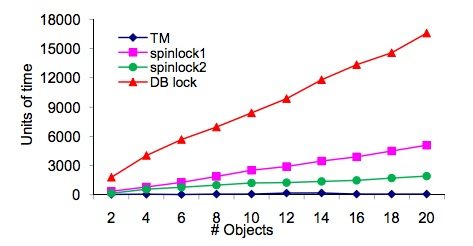
\includegraphics[width=0.45\textwidth]{figure/overhead.jpg} \caption{Overhead
%of different concurrency control protocols under low contention workloads
%\citep{tran2010}.} \label{fig:overhead} \end{figure}

\section{Project Plan} \label{sec:plan}

Broadly speaking, we plan to:
\begin{itemize}
\item implement two different TSX-based concurrency control schemes for a simple key-value store
\item evaluate the performance of that concurrency control scheme under different workloads
\end{itemize}
The goals of the project are as follows:
\begin{itemize}
\item \textbf{75\% goal:} Implement concurrency control for a key-value store with both HLE and RTM, and compare the performance of these two schemes against each other.
\item \textbf{100\% goal:} Additionally, compare the above approaches with traditional pessimistic concurrency control schemes, specifically spin-locks and a basic lock manager. This will demonstrate the advantages of the hardware-based approach for this task, or else show that this task is not one where the hardware-based approach helps.
\item \textbf{125\% goal:} Additionally, implement a software-based (i.e., timestamp-based) OCC scheme and compare it against the above approaches. This will serve as a basic check that it is in fact the hardware that is the cause of any differences in performance, not just the optimistic approach to concurrency.
\end{itemize}

\subsection{Resources Required}
The only resource absolutely necessary for this project is access to a machine with a Haswell processor. Dong has granted us access to a CMU-owned machine.

It would be useful, though not essential, to have access to the existing codebase that has been used by Professor Andersen's lab to run similar HTM experiments in the past. In particular, it would be helpful to have access to the key-value store implementation used in the lab's in-progress study. We are expecting that Dong will be able to give us access to this, as well.

\subsection{Experiments}
Our experiments are inspired by those reported in \citep{tran2010}. We will restrict ourselves to a small, fixed number of key-value store entries. In each experiment, we will measure the time it takes to run a randomly generated workload of datastore operations, given a particular CC scheme. Each workload will simply consist of looking up some set of keys and trivially modifying their values (e.g., incrementing). Specifically, we will run the following experiments for each type of CC mechanism:
\begin{enumerate}
\item With several fixed sizes for read/write sets and numbers of threads, vary the contention level between operations on different threads. This will allow us to determine how each of the CC mechanisms scales with respect to contention.
\item With several different fixed contention levels and numbers of threads, vary the size of the read/write sets. This will allow us to determine how each of the CC mechanisms scales with respect to the read/write set. (For HTM, this may be a very important factor, since transactions abort based on conflicts anywhere in the read/write set.)
\item With several different fixed contention levels and read/write set sizes, vary the number of threads running. This will allow us to determine how much benefit each mechanism is able to benefit from adding more parallelism.
\end{enumerate}

\subsection{Work Plan}
The required steps for executing this project are as follows:
\begin{enumerate}
\item Familiarize ourselves with an existing basic key-value store system, such as that built by Professor Andersen's group, or (if that turns out to be impractical) implement our own. If we end up choosing the latter approach, we can minimize implementation effort by keeping the data structures very simple -- just 1-2 hash tables, one for the data and one for locks or to group data entries larger than a cache line (if applicable).
\item Design the structure of the transaction manager to support multiple CC mechanisms.
\item Using the Haswell TSX APIs, implement a transaction manager that optimistically attempts to execute a transaction, and retries according to either an HLE strategy or a custom RTM-specified strategy.
\item Write a system to generate test workloads with different amounts of contention. It should also allow specifying thread assignments if necessary.
\item Run the experiments for the two HTM approaches. Some tweaking will be necessary to find the most informative thread numbers, read/write set sizes, and contention levels.
\item Implement spin-locks and a lock manager.
\item Rerun the experiments for the pessimistic concurrency control approaches.
\item Implement software-based OCC.
\item Rerun the experiments for OCC.
\item Collate/visualize data and write up report.
\end{enumerate}

All of us will work together on items 1 and 2. Two of us (jdunietz and jarulraj) will collaborate (via pair programming) to implement the TSX-based transaction manager. In parallel, twmarsha will implement the workload generator using an agreed-upon interface. jarulraj and twmarsha will each run preliminary versions of one experiment for item 5, and jdunietz will use their results to run the final experiments and collate/visualize the data. twmarsha will implement a lock manager, jarulraj will implement spin-locks, and jdunietz will implement OCC.


\bibliographystyle{plain}
\bibliography{ref}

\end{document}
% end doc
